\begin{exercise}{2016/17 10}
    \emph{Σταθεροποίηση του σαγματικού σημείου του εκκρεμούς}: Θα αναλύσουμε
    κάποιες μεθόδους \enquote*{εξισορρόπησης} του εκκρεμούς στην κάθετη προς τα
    πάνω θέση (χωρίς να ισχυριζόμαστε ότι είναι ιδιαίτερα χρήσιμες στην πράξη).

    Οι εξισώσεις είναι, όπως και πριν:
    \begin{align*}
        \dot{x} &= y \\
        \dot{y} &= -a y - \sin{x}
    \end{align*}
    για \( a \) θετικό και μικρό (π.χ. \( a = 0.3 \)).
    \begin{enumerate}[label= (\alph*)]
        \item Θεωρούμε έλεγχο που επεισέρχεται στην εξίσωση για τη γωνία, δηλαδή
            θεωρούμε τη νέα πρώτη εξίσωση:
            \[
                \dot{x} = y + u_1(x).
            \]
            Βρείτε τον έλεγχο \( u_1(x) = -kx + c \) ο οποίος σταθεροποιεί το
            σαγματικό σημείο \( (x, y) = (\pi, 0) \), δηλαδή να έχει το σημείο
            αυτό ως ολικό ελκυστή (ασυμπτωτικά ευσταθές σημείο ισορροπίας).
            Είναι δυνατό αυτό εάν το σύστημα είναι χωρίς απώλειες
            (δηλαδή \( a = 0 \));
        \item Επαναλάβετε για έλεγχο στη γωνιακή ταχύτητα, δηλαδή με νέα δεύτερη
            εξίσωση:
            \[
                \dot{y} = -ay -\sin{x} + u_2(x),
            \]
            πάλι με \( u_2(x) = -kx + c \).
    \end{enumerate}
    Και στις δύο περιπτώσεις, δώστε κατάλληλα πορτρέτα κίνησης του ελεγχόμενου
    συστήματος που επιλέξατε.
\end{exercise}
\begin{solution}
    (α). Με τον έλεγχο \( u_1(x) \) οι εξισώσεις είναι
    \begin{align*}
        \dot{x} &= y -kx + c\\
        \dot{y} &= -a y - \sin{x}.
    \end{align*}
    Εφόσον θέλουμε το σημείο \( (\pi, 0) \) να είναι ασυμπτωτικά ευσταθές,
    μπορούμε από τη γραμμικοποίηση να βρούμε τις συνθήκες για το \( k \) που θα
    επιτυγχάνει το στόχο αυτόν. Έτσι έχουμε
    \[
        \begin{pmatrix}
            \dot{x} \\
            \dot{y}
        \end{pmatrix} = F(x, y) =
        \begin{pmatrix}
            y -kx + c \\
            -a y - \sin{x}
        \end{pmatrix}.
    \]
    Η γραμμικοποίηση είναι
    \[
        DF(x, y) =
        \begin{pmatrix}
            -k & 1 \\
            -\cos{x} & -a
        \end{pmatrix},
    \]
    και στο σημείο \( (\pi, 0) \) έχουμε
    \[
        DF(\pi, 0) =
        \begin{pmatrix}
            -k & 1 \\
            1 & -a
        \end{pmatrix}.
    \]
    Εφόσον θέλουμε ασυμπτωτική ευστάθεια, θα πρέπει \(
    \operatorname{Re}(\lambda) < 0 \). Άρα οι ιδιοτιμές είναι
    \begin{align*}
        \det{\begin{pmatrix}
                -k - \lambda & 1 \\
                1 & -a - \lambda
        \end{pmatrix}} &=
        (-k - \lambda)(-a - \lambda) - 1 \\
        &= ka + k\lambda + \lambda a + \lambda^2 - 1 \\
        &= \lambda^2 + \lambda(k + a) + ka - 1.
    \end{align*}
    Η διακρίνουσα της παραπάνω είναι
    \begin{align*}
        \Delta &= (k + a)^2 - 4(ka - 1) \\
        &= k^2 + a^2 + 2ka - 4ka + 4 \\
        &= (k - a)^2 + 4 > 0.
    \end{align*}
    Συνεπώς, έχουμε δύο διακριτές πραγματικές ιδιοτιμές. Επομένως πρέπει
    \[
        \lambda = \frac{-(k + a) \pm\sqrt{(k -a)^2 + 4}}{2} < 0.
    \]
    Έστω \( \lambda_1 \) η ιδιοτιμή που αντιστοιχεί όταν μπροστά από την
    τετραγωνική ρίζα έχουμε το θετικό πρόσημο και \( \lambda_2 \) η ιδιοτιμή
    που αντιστοιχεί όταν μπροστά από την τετραγωνική ρίζα έχουμε το αρνητικό
    πρόσημο.

    Οι ρίζες της \( \lambda_1 \) είναι
    \[
        -(k + a) + \sqrt{(k -a)^2 + 4} = 0,
    \]
    που συνεπάγεται
    \begin{align*}
         \sqrt{(k -a)^2 + 4} &= (k + a) \\
         (k -a)^2 + 4 &= (k + a)^2 \\
         k^2 + a^2 -2ka + 4 &= k^2 + a^2 + 2ka \\
         -4ka &= -4 \\
         k &= \frac{1}{a}. \\
    \end{align*}
    Άρα για την ιδιοτιμή \( \lambda_1 \) πρέπει
    \begin{equation}\label{eq:ex10_a_lambda_1}
        \lambda_1 < 0 \Rightarrow k > \frac{1}{a}.
    \end{equation}
    Ομοίως για την ιδιοτιμή \( \lambda_2 \) πρέπει
    \[
        -(k + a) - \sqrt{(k -a)^2 + 4} < 0,
    \]
    που όμως αρκεί
    \begin{align*}
        -(k + a) &< 0 \\
        -k &< a.
    \end{align*}
    Άρα για την ιδιοτιμή \( \lambda_2 \) πρέπει
    \[
        \lambda_2 < 0 \Rightarrow k > -a,
    \]
    η οποία όμως είναι περιττή καθώς εμπεριέχεται από την ανισότητα της
    σχέσης~\eqref{eq:ex10_a_lambda_1}.

    Δηλαδή για \( k > 1/a \) και οριακά για \( k = 1/a \) το σύστημα, η
    συνιστώσα \( x \) (θέση), θα ισορροπήσει στο σαγματικό σημείο ισορροπίας
    \( (\pi, 0) \) το οποίο θα είναι ασυμπτωτικά ευσταθές. Το πόσο γρήγορα θα
    φτάσουμε στο στόχο μας εξαρτάται από την απόλυτη τιμή των ιδιοτιμών. Έτσι
    για \( k = 1/a \) θα φτάσουμε το στόχο, αλλά \enquote*{αργά}. Όσο αυξάνεται
    το \( k \) τόσο πιο γρήγορα θα ισορροπήσει η θέση στη γωνία \( \pi \).

    Από τη συνθήκη για το \( k \), η ανισότητα της
    σχέσης~\eqref{eq:ex10_a_lambda_1}, φαίνεται ότι όσο μικραίνει η απόσβεση,
    τόσο μεγαλύτερο πρέπει να γίνει το \( k \). Για την οριακή τιμή \( a = 0 \)
    τότε \( k \to \infty \) και άρα το να ισορροπήσουμε το σύστημα στη θέση \(
    (\pi, 0) \) είναι αδύνατο.

    Στο σχήμα~\ref{fig:ex10_invPend15a} παρουσιάζεται η χρονική απόκριση του
    εκκρεμούς με αρχικές συνθήκες \( (0, 0) \), για μικρή απόσβεση \( a = 0.3 \)
    και έλεγχο
    \[
        u_1(x) = -\frac{1.5}{a}x + \frac{1.5}{a}\pi.
    \]
    Το μικρό κέρδος όπως βλέπουμε, παρόλο που καταφέρνει να ισορροπήσει το
    σύστημα στο \( (\pi, 0) \) απαιτεί πολύ χρόνο.
    \begin{figure}[h!]
        \centering
        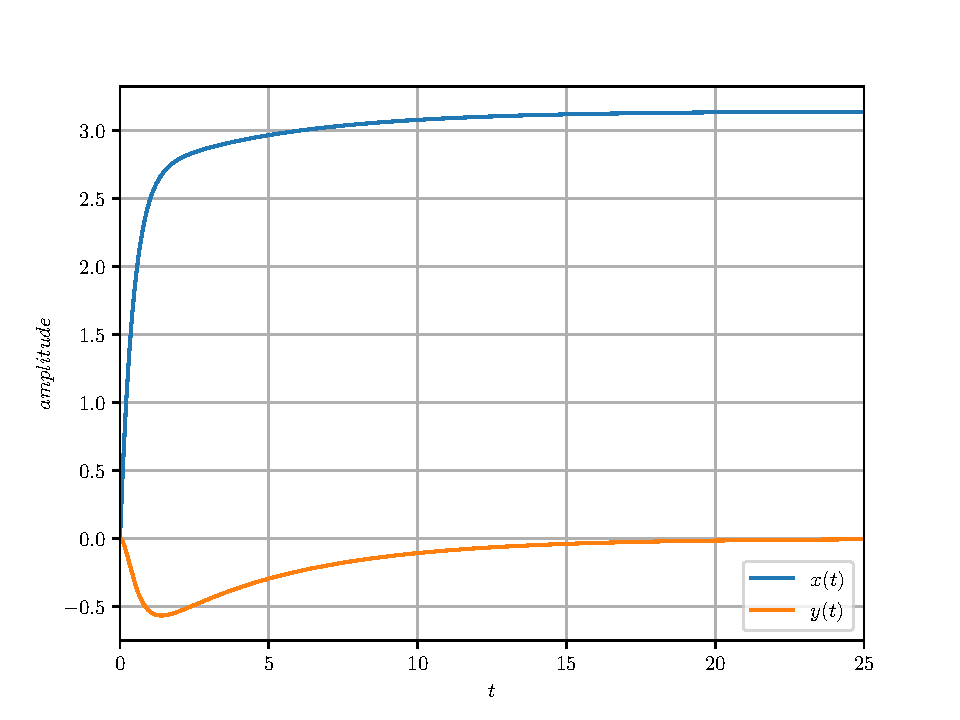
\includegraphics[width=0.9\textwidth]{figures/ex10_invPend15a.pdf}
        \caption{\gr{Χρονική απόκριση ανάστροφου εκκρεμούς,
        \( k = 1.5/a, a = 0.3 \)}}
        \label{fig:ex10_invPend15a}
    \end{figure}
    \begin{figure}[h!]
        \centering
        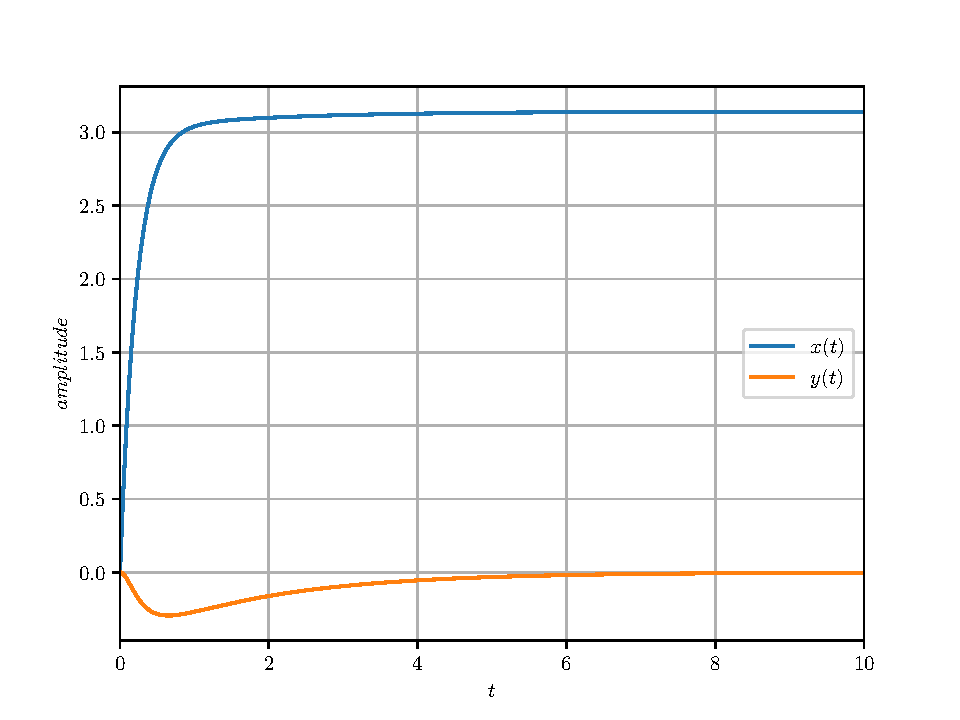
\includegraphics[width=0.9\textwidth]{figures/ex10_invPend35a.pdf}
        \caption{\gr{Χρονική απόκριση ανάστροφου εκκρεμούς,
        \( k = 3.5/a, a = 0.3 \)}}
        \label{fig:ex10_invPend35a}
    \end{figure}
    Στο σχήμα~\ref{fig:ex10_invPend35a} παρουσιάζεται η χρονική απόκριση του
    εκκρεμούς με αρχικές συνθήκες \( (0, 0) \), για μικρή απόσβεση \( a = 0.3 \) και έλεγχο
    \[
        u_1(x) = -\frac{3.5}{a}x + \frac{3.5}{a}\pi.
    \]
    Στην περίπτωση αυτή το σύστημα ισορροπεί πολύ πιο γρήγορα. Δεδομένου ότι στο
    παράδειγμα δεν έχουμε κάποιο δείκτη επίδοσης που να περιορίζει τις τιμές του
    \( k \) είμαστε ελεύθεροι να τις επιλέξουμε όσο μεγάλες επιθυμούμε. Παρόλα
    αυτά μία τιμή του \( k \) σε αυτή την περιοχή φαίνεται αρκετά λογική γιατί
    στην πράξη ο έλεγχος θα είναι πάντα φραγμένος.

    Στο σχήμα~\ref{fig:ex10_invPend35aComb} παρουσιάζεται το πορτρέτο κίνησης
    για \( k = 3.5/a, a = 0.3 \).
    \begin{figure}[h]
        \centering
        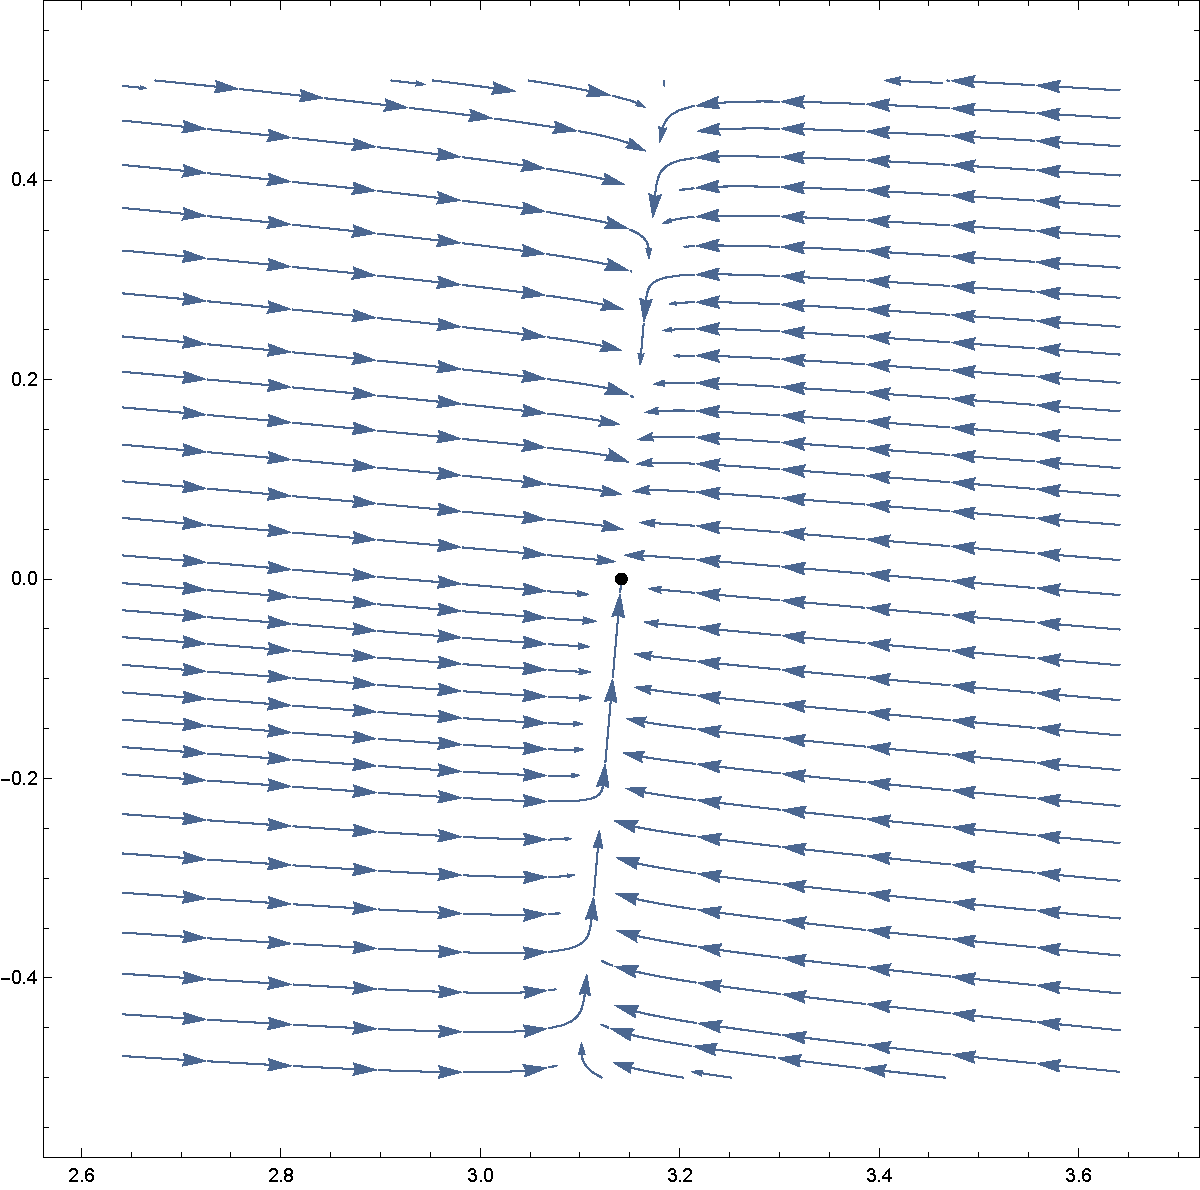
\includegraphics[width=0.8\textwidth]{figures/ex10_invPend35aComb.pdf}
        \caption{\gr{Πορτρέτο κίνησης ανάστροφου εκκρεμούς,
        \( k = 3.5/a, a = 0.3 \)}}
        \label{fig:ex10_invPend35aComb}
    \end{figure}

    (β). Με τον έλεγχο \( u_2(x) \) οι εξισώσεις είναι
    \begin{align*}
        \dot{x} &= y \\
        \dot{y} &= -a y - \sin{x} - kx + c.
    \end{align*}
    Εφόσον θέλουμε το σημείο \( (\pi, 0) \) να είναι ασυμπτωτικά ευσταθές,
    μπορούμε από τη γραμμικοποίηση να βρούμε τις συνθήκες για το \( k \) που θα
    επιτυγχάνει το στόχο αυτόν. Έτσι έχουμε
    \[
        \begin{pmatrix}
            \dot{x} \\
            \dot{y}
        \end{pmatrix} = F(x, y) =
        \begin{pmatrix}
            y -kx + c \\
            -a y - \sin{x}
        \end{pmatrix}.
    \]
    Η γραμμικοποίηση είναι
    \[
        DF(x, y) =
        \begin{pmatrix}
            0 & 1 \\
            -\cos{x} - k & -a
        \end{pmatrix},
    \]
    και στο σημείο \( (\pi, 0) \) έχουμε
    \[
        DF(\pi, 0) =
        \begin{pmatrix}
            0 & 1 \\
            1 - k & -a
        \end{pmatrix}.
    \]
    Εφόσον θέλουμε ασυμπτωτική ευστάθεια, θα πρέπει \(
    \operatorname{Re}(\lambda) < 0 \). Άρα οι ιδιοτιμές είναι
    \begin{align*}
        \det{\begin{pmatrix}
                -\lambda & 1 \\
                1 - k & -a - \lambda
        \end{pmatrix}} &=
        -\lambda)(-a - \lambda) - 1 + k \\
        &= \lambda a + \lambda^2 - 1 + k \\
        &= \lambda^2 + \lambda a - 1 + k.
    \end{align*}
    Η διακρίνουσα της παραπάνω είναι
    \[
        \Delta = a^2 - 4(-1 + k) = a^2 + 4(1 - k).
    \]
    Η ρίζα της διακρίνουσας είναι
    \begin{align*}
        a^2 + 4(1 - k) &= 0 \\
        1 - k &= -\frac{a^2}{4},
    \end{align*}
    που σημαίνει
    \[
        k = 1 + \frac{a^2}{4}.
    \]
    Άρα έχουμε
    \[
        \Delta > 0 \Rightarrow k < 1 + \frac{a^2}{4}, \quad
        \Delta < 0 \Rightarrow k > 1 + \frac{a^2}{4}, \quad
        \Delta = 0 \Rightarrow k = 1 + \frac{a^2}{4}.
    \]
    Οι ιδιοτιμές δίνονται από τη σχέση
    \begin{equation}\label{eq:ex10b_lambda}
        \lambda = \frac{-a \pm\sqrt{a^2 + 4(1 - k)}}{2},
    \end{equation}
    και θα πάρουμε περιπτώσεις για να βρούμε τις συνθήκες για το \( k \).

    Έστω \( \lambda_1 \) η ιδιοτιμή που αντιστοιχεί όταν μπροστά από την
    τετραγωνική ρίζα έχουμε το θετικό πρόσημο και \( \lambda_2 \) η ιδιοτιμή
    που αντιστοιχεί όταν μπροστά από την τετραγωνική ρίζα έχουμε το αρνητικό
    πρόσημο.

    Αν δούμε αρχικά την περίπτωση που \( \Delta > 0 \), τότε προφανώς η \(
    \lambda_2 < 0 \), άρα μένει να κοιτάξουμε την \( \lambda_1 \). Για να είναι
    αυτή αρνητική πρέπει
    \begin{align*}
        -a + \sqrt{a^2 + 4(1 - k)} &< 0 \\
        a^2 + 4(1 - k) < a^2,
    \end{align*}
    που σημαίνει
    \[
        k < 1.
    \]
    Προφανώς η παραπάνω εμπεριέχει την προηγούμενη συνθήκη ώστε η διακρίνουσα να
    είναι θετική. Άρα για \( k < 1 \) το \( (\pi, 0) \) είναι ασυμπτωτικά
    ευσταθές και έχει τη μορφή ευσταθούς κόμβου.

    Όταν \( \Delta < 0 \), κοιτώντας τη σχέση~\eqref{eq:ex10b_lambda}, επειδή το
    πραγματικό μέρος είναι πάντα αρνητικό αυτό σημαίνει ότι το \( (\pi, 0) \) σημείο
    είναι ασυμπτωτικά ευσταθές με μορφή ευσταθούς εστίας.

    Τέλος, όταν \( \Delta = 0 \), έχουμε διπλή ρίζα και ιδιοτιμές \(
    \lambda_{1,2} = -a/2 \) και το \( (\pi, 0) \) σημείο είναι ασυμπτωτικά
    ευσταθές.

    Στο σχήμα~\ref{fig:ex10_b_invPend4a} παρουσιάζεται η χρονική απόκριση του
    εκκρεμούς με αρχικές συνθήκες \( (0, 0) \), για μικρή απόσβεση \( a = 0.3 \)
    και έλεγχο
    \[
        u_2(x) = -4\left(1 + \frac{a^2}{4}\right)x +
        4\left(1 + \frac{a^2}{4}\right)\pi,
    \]
    και στο σχήμα~\ref{fig:ex10_b_invPend4Comb} το αντίστοιχο πορτρέτο κίνησης.
    \begin{figure}[h]
        \centering
        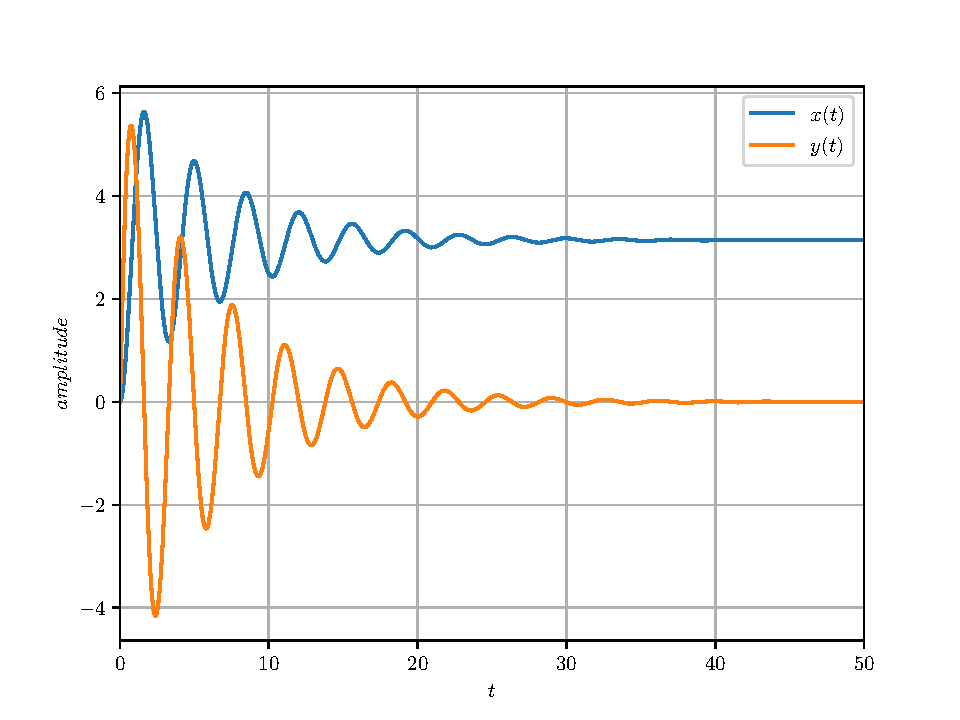
\includegraphics[width=0.9\textwidth]{figures/ex10_b_invPend4a.pdf}
        \caption{\gr{Χρονική απόκριση ανάστροφου εκκρεμούς,
        \( k = 4(1 + a^2/4), a = 0.3 \)}}
        \label{fig:ex10_b_invPend4a}
    \end{figure}
    \begin{figure}[h]
        \centering
        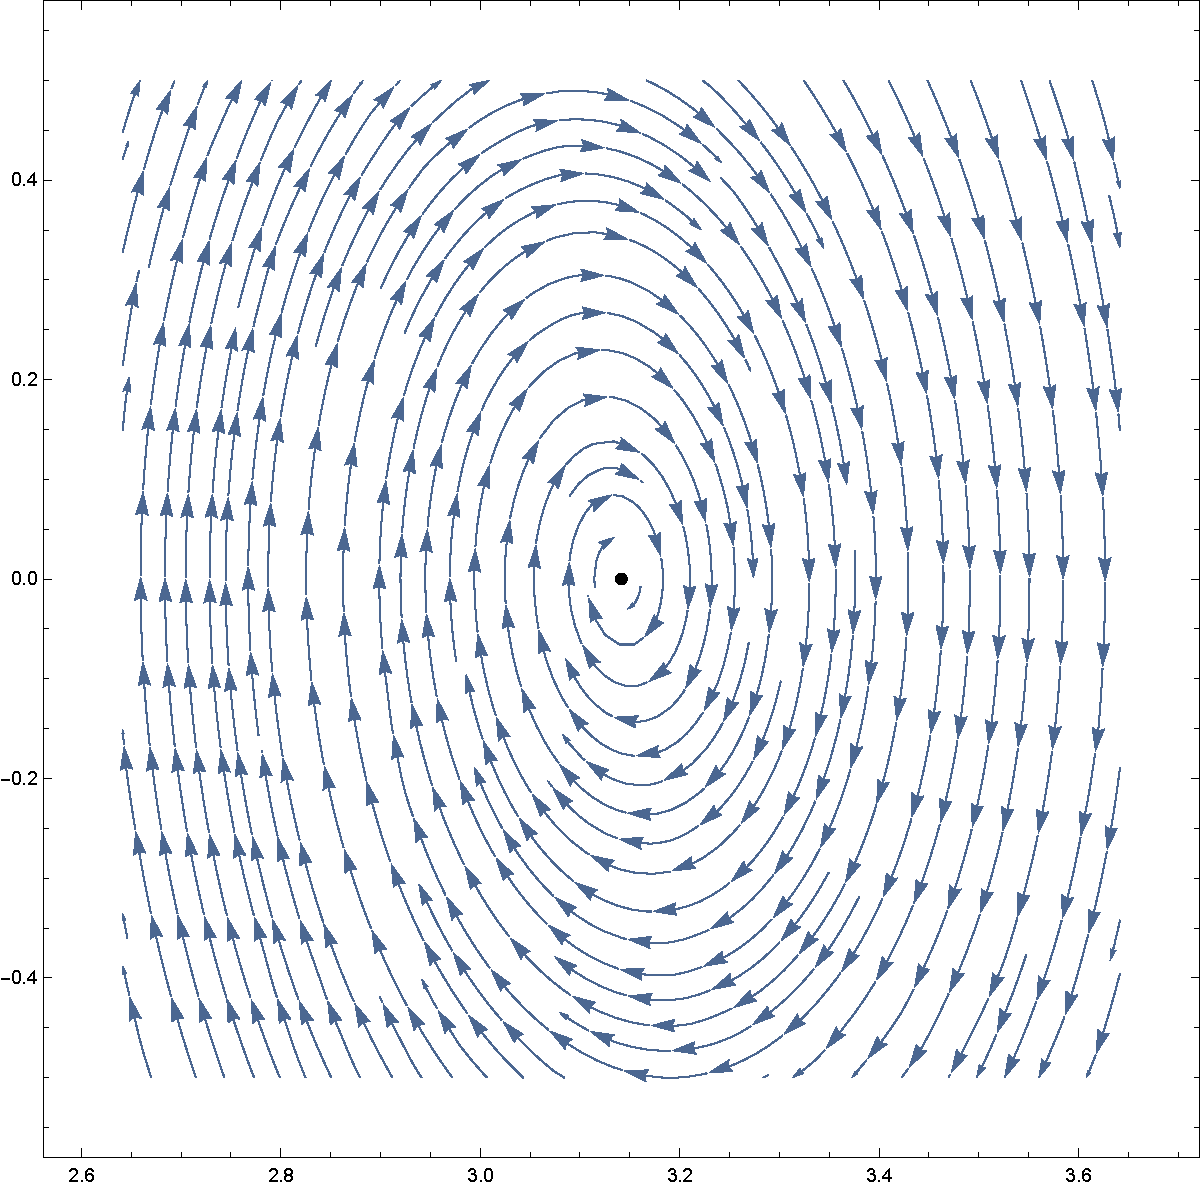
\includegraphics[width=0.8\textwidth]{figures/ex10_b_invPend4Comb.pdf}
        \caption{\gr{Πορτρέτο κίνησης ανάστροφου εκκρεμούς,
        \( k = 4(1 + a^2/4), a = 0.3 \)}}
        \label{fig:ex10_b_invPend4Comb}
    \end{figure}
    Είναι προφανές ότι βρισκόμαστε στην περιοχή της ευσταθής εστίας. Από τα
    διαγράμματα παρατηρούμαι ότι ο στόχος είναι αρκετά δυσκολότερος. Η μικρή
    απόσβεση δημιουργεί μεγάλες ταλαντώσεις στον έλεγχο της ταχύτητας του
    εκκρεμούς. Μεγαλώνοντας το κέρδος \( k \) θα φτάσουμε συντομότερα στο σημείο
    \( (\pi, 0) \), άλλα θα εμφανιστούν ακόμα μεγαλύτερες ταλαντώσεις. Ιδανικά
    θα επιλέγαμε μία απόσβεση με τιμές γύρω στο \( 0.8 - 0.9 \) για καλύτερες
    αποδόσεις.

    Στο σχήμα~\ref{fig:ex10_b_invPendll} παρουσιάζεται η χρονική απόκριση του
    εκκρεμούς με αρχικές συνθήκες \( (0, 0) \), για μικρή απόσβεση \( a = 0.3 \)
    και έλεγχο
    \[
        u_2(x) = -\left(1 + \frac{a^2}{4}\right)x +
        \left(1 + \frac{a^2}{4}\right)\pi,
    \]
    και στο σχήμα~\ref{fig:ex10_b_invPendllComb} το αντίστοιχο πορτρέτο κίνησης.
    \begin{figure}[h]
        \centering
        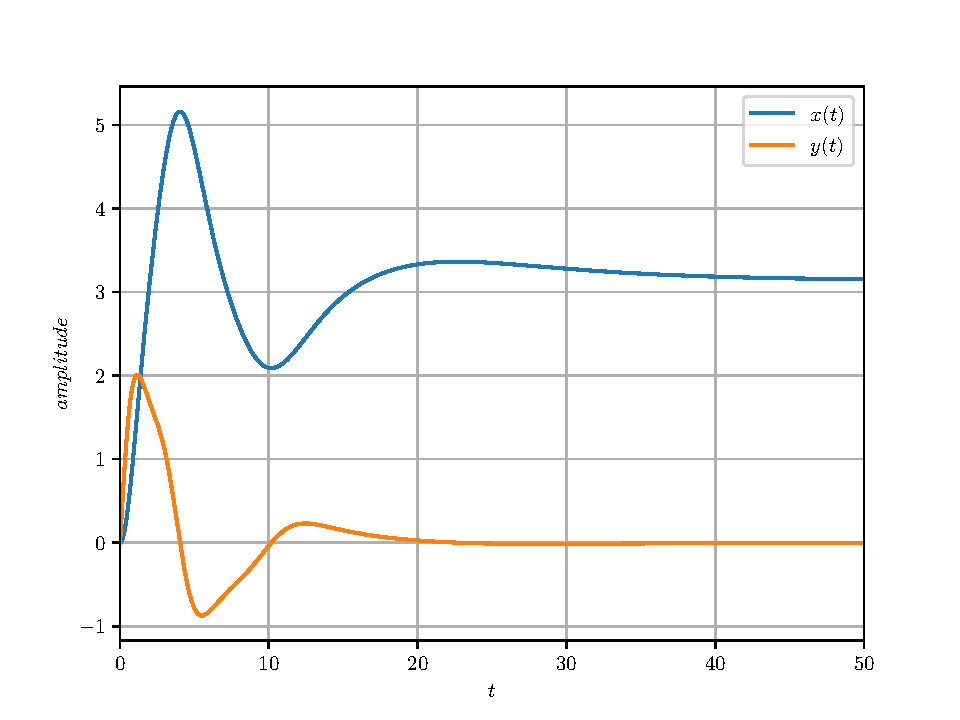
\includegraphics[width=0.9\textwidth]{figures/ex10_b_invPendll.pdf}
        \caption{\gr{Χρονική απόκριση ανάστροφου εκκρεμούς,
        \( k = 1 + a^2/4, a = 0.3 \)}}
        \label{fig:ex10_b_invPendll}
    \end{figure}
    \begin{figure}[h]
        \centering
        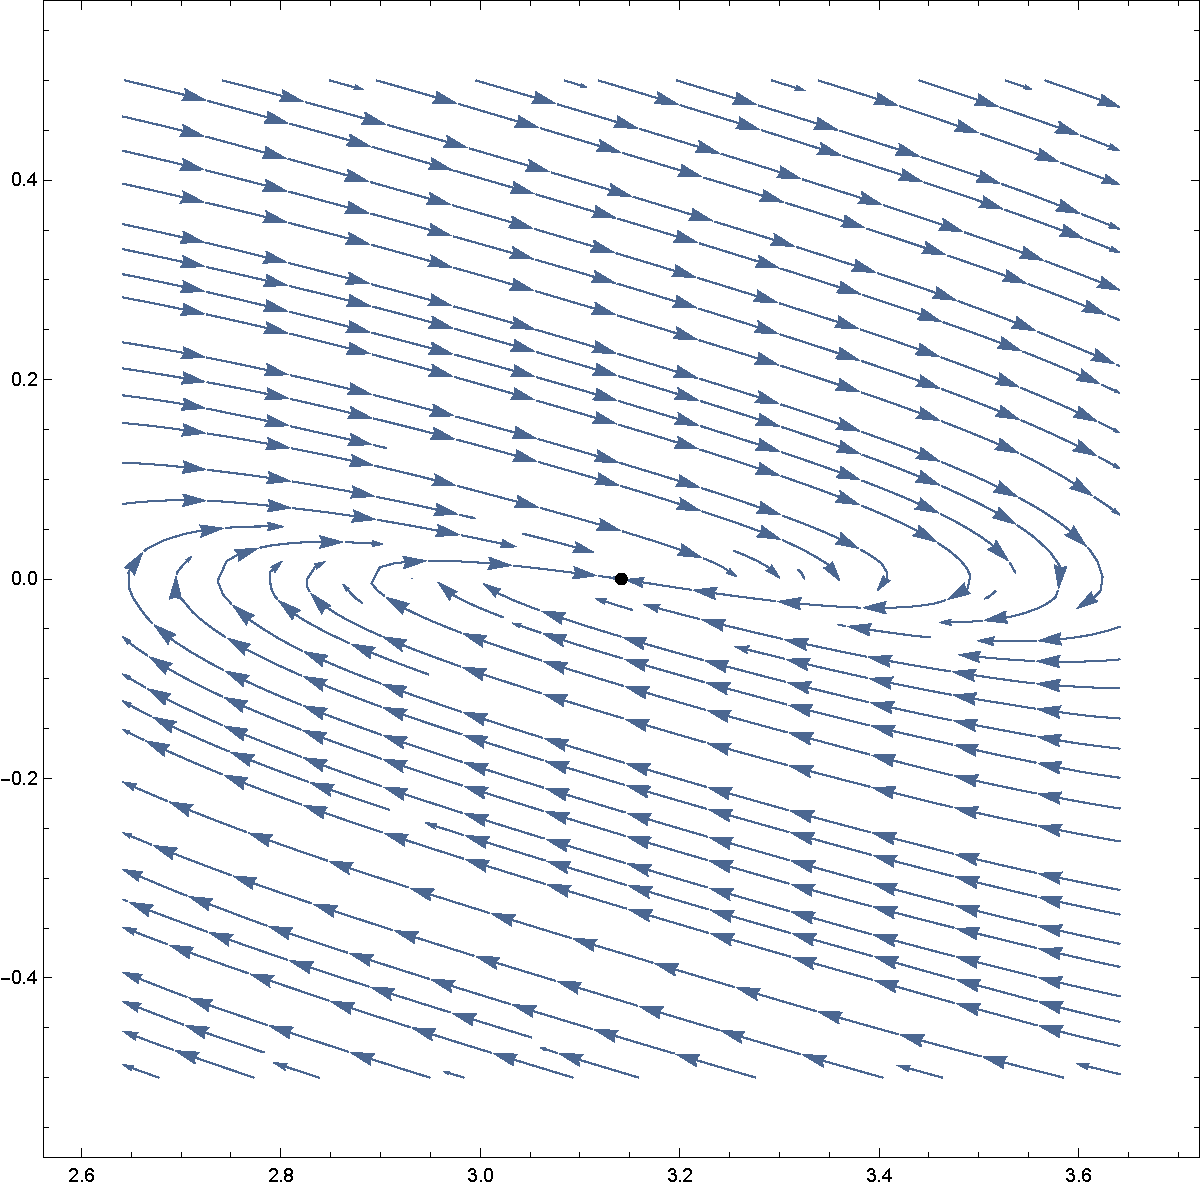
\includegraphics[width=0.8\textwidth]{figures/ex10_b_invPendllComb.pdf}
        \caption{\gr{Πορτρέτο κίνησης ανάστροφου εκκρεμούς,
        \( k = 1 + a^2/4, a = 0.3 \)}}
        \label{fig:ex10_b_invPendllComb}
    \end{figure}
    Το παράδειγμα αυτό παρουσιάζεται απλώς για επιβεβαίωση των υπολογισμών.
    Παρατηρούμε πως το \( (\pi, 0) \) είναι ασυμπτωτικά ευσταθές και έχει τη
    μορφή διπλής ρίζας.
\end{solution}
